\subsection{Solution}

\subsection{Online Clustering}

Detecting events in a stream of news articles will be achieved by using an online clustering approach. The events of interest for this application are the discovery of new topics and the extension of existing topics. Thus we define our two events as follows:

\begin{itemize}
    \item Topic added: A new cluster of news articles appears in the data stream.
    \item Topic extended: An existing topic is extended by additional news articles.
\end{itemize}

HDBSCAN will be applied as the clustering method, using the optimal settings as discovered in the preivous evaluation. Additional preprocessing of news articles before clustering is going to be explored as part of evaluation as well and will be implemented accordingly for the online clustring.

Since HDBSCAN only supports static datasets, the clustering will be done in batches using a time based sliding window approach. Events are detected by comparing the resulting clusters with the previous ones.

\begin{figure}[h]
    \centering

    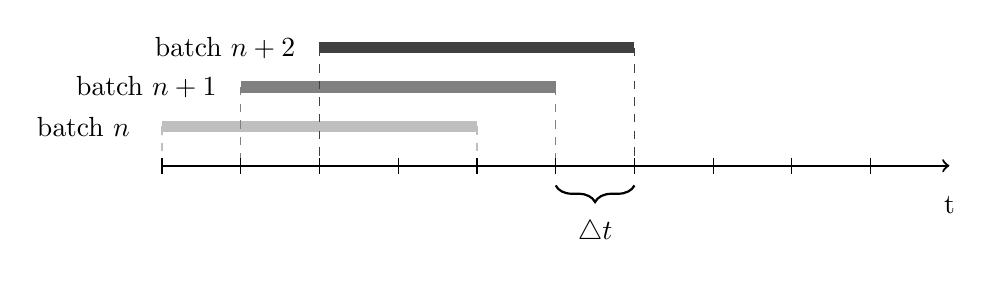
\begin{tikzpicture}[scale=1]


        \draw[lightgray, line width=4pt] (0,.5) -- (4,.5);
        \draw[lightgray, dashed] (0,.5) -- (0,0);
        \draw[lightgray, dashed] (4,.5) -- (4,0);
        \node[align=right] at (-1,.5) {batch $n$};

        \draw[gray, line width=4pt] (1,1) -- (5,1);
        \draw[gray, dashed] (1,1) -- (1,0);
        \draw[gray, dashed] (5,1) -- (5,0);
        \node[align=right] at (-.2,1) {batch $n + 1$};

        \draw[darkgray, line width=4pt] (2,1.5) -- (6,1.5);
        \draw[darkgray, dashed] (2,1.5) -- (2,0);
        \draw[darkgray, dashed] (6,1.5) -- (6,0);
        \node[align=right] at (0.8,1.5) {batch $n + 2$};

        \node[align=center] at (5.5,-0.85) {$\triangle t$};
        \node[align=center] at (10,-0.5) {t};

        \draw [thick,->] (0,0) -- (10,0);
        \foreach \x in {0,...,9} \draw (\x,0.1) -- (\x,-0.1);

        \draw [thick,decorate,decoration={brace,amplitude=6pt,raise=0pt,mirror}] (5,-0.25) -- (6,-0.25);

        \end{tikzpicture}

    \caption{Timeline showing the sliding window approach}
    \label{fig:timeline}
\end{figure}

\subsubsection{Finding pairs clusters}

To be able to compare clusters of different batches with each other, we have to find pairs of clusters between batches, which describe the same topic. This is done by applying the same assumptions as for the scoring function used in the evaluation. Therefore clusters are paired based on their similarity calculated with the jaccard index as shown in equation \ref{equ:similarity}. If the similarity is above a certain threshold, both clusters are seen as describing the same topic.

\subsubsection{Sliding window}

An important consideration for determining existing or new clusters is the overlap of samples between batches. If the overlap is too small, similar clusters will no longer be detected as such, which would result in an increasingly high error rate. Finding optimal values for the step size between batches and the number of samples for each batch is therefore essential for our online clustering approach.
